\documentclass{beamer}
\usepackage{amsmath}
\usepackage[english]{babel} %set language; note: after changing this, you need to delete all auxiliary files to recompile
\usepackage[utf8]{inputenc} %define file encoding; latin1 is the other often used option
\usepackage{csquotes} % provides context sensitive quotation facilities
\usepackage{graphicx} %allows for inserting figures
\usepackage{booktabs} % for table formatting without vertical lines
\usepackage{textcomp} % allow for example using the Euro sign with \texteuro
\usepackage{stackengine}
\usepackage{wasysym}
\usepackage{tikzsymbols}
\usepackage{textcomp}
% ELIMINAR COMANDOS DE NAVEGACION%%%%%%%%%%%
\setbeamertemplate{navigation symbols}

%\newcommand{\bubblethis}[2]{
 %       \tikz[remember picture,baseline]{\node[anchor=base,inner sep=0,outer sep=0]%
 %       (#1) {\underline{#1}};\node[overlay,cloud callout,callout relative pointer={(0.2cm,-0.7cm)},%
 %       aspect=2.5,fill=yellow!90] at ($(#1.north)+(-0.5cm,1.6cm)$) {#2};}%
 %   }%
%\tikzset{face/.style={shape=circle,minimum size=4ex,shading=radial,outer sep=0pt,
 %       inner color=white!50!yellow,outer color= yellow!70!orange}}

%% Some commands to make the code easier
\newcommand{\emoticon}[1][]{%
  \node[face,#1] (emoticon) {};
  %% The eyes are fixed.
  \draw[fill=white] (-1ex,0ex) ..controls (-0.5ex,0.2ex)and(0.5ex,0.2ex)..
        (1ex,0.0ex) ..controls ( 1.5ex,1.5ex)and( 0.2ex,1.7ex)..
        (0ex,0.4ex) ..controls (-0.2ex,1.7ex)and(-1.5ex,1.5ex)..
        (-1ex,0ex)--cycle;}
\newcommand{\pupils}{
  %% standard pupils
  \fill[shift={(0.5ex,0.5ex)},rotate=80] 
       (0,0) ellipse (0.3ex and 0.15ex);
  \fill[shift={(-0.5ex,0.5ex)},rotate=100] 
       (0,0) ellipse (0.3ex and 0.15ex);}

\newcommand{\emoticonname}[1]{
  \node[below=1ex of emoticon,font=\footnotesize,
        minimum width=4cm]{#1};}
\usepackage{scalerel}
\usetikzlibrary{positioning}
\usepackage{xcolor,amssymb}
\newcommand\dangersignb[1][2ex]{%
  \scaleto{\stackengine{0.3pt}{\scalebox{1.1}[.9]{%
  \color{red}$\blacktriangle$}}{\tiny\bfseries !}{O}{c}{F}{F}{L}}{#1}%
}
\newcommand\dangersignw[1][2ex]{%
  \scaleto{\stackengine{0.3pt}{\scalebox{1.1}[.9]{%
  \color{red}$\blacktriangle$}}{\color{white}\tiny\bfseries !}{O}{c}{F}{F}{L}}{#1}%
}
\usepackage{fontawesome} % Social Icons
\usepackage{epstopdf} % allow embedding eps-figures
\usepackage{tikz} % allows drawing figures
\usepackage{amsmath,amssymb,amsthm} %advanced math facilities
\usepackage{lmodern} %uses font that support italic and bold at the same time
\usepackage{hyperref}
\usepackage{tikz}
\hypersetup{
    colorlinks=true,
    linkcolor=blue,
    filecolor=magenta,      
    urlcolor=blue,
}
\usepackage{tcolorbox}
%add citation management using BibLaTeX
\usepackage[citestyle=authoryear-comp, %define style for citations
    bibstyle=authoryear-comp, %define style for bibliography
    maxbibnames=10, %maximum number of authors displayed in bibliography
    minbibnames=1, %minimum number of authors displayed in bibliography
    maxcitenames=3, %maximum number of authors displayed in citations before using et al.
    minnames=1, %maximum number of authors displayed in citations before using et al.
    datezeros=false, % do not print dates with leading zeros
    date=long, %use long formats for dates
    isbn=false,% show no ISBNs in bibliography (applies only if not a mandatory field)
    url=false,% show no urls in bibliography (applies only if not a mandatory field)
    doi=false, % show no dois in bibliography (applies only if not a mandatory field)
    eprint=false, %show no eprint-field in bibliography (applies only if not a mandatory field)
    backend=biber %use biber as the backend; backend=bibtex is less powerful, but easier to install
    ]{biblatex}
\addbibresource{../mybibfile.bib} %define bib-file located one folder higher


\usefonttheme[onlymath]{serif} %set math font to serif ones

\definecolor{beamerblue}{rgb}{0.2,0.2,0.7} %define beamerblue color for later use

%%% defines highlight command to set text blue
\newcommand{\highlight}[1]{{\color{blue}{#1}}}


%%%%%%% commands defining backup slides so that frame numbering is correct

\newcommand{\backupbegin}{
   \newcounter{framenumberappendix}
   \setcounter{framenumberappendix}{\value{framenumber}}
}
\newcommand{\backupend}{
   \addtocounter{framenumberappendix}{-\value{framenumber}}
   \addtocounter{framenumber}{\value{framenumberappendix}}
}

%%%% end of defining backup slides

%Specify figure caption, see also http://tex.stackexchange.com/questions/155738/caption-package-not-working-with-beamer
\setbeamertemplate{caption}{\insertcaption} %redefines caption to remove label "Figure".
%\setbeamerfont{caption}{size=\scriptsize,shape=\itshape,series=\bfseries} %sets figure  caption bold and italic and makes it smaller


\usetheme{Boadilla}

%set options of hyperref package
\hypersetup{
    bookmarksnumbered=true, %put section numbers in bookmarks
    naturalnames=true, %use LATEX-computed names for links
    citebordercolor={1 1 1}, %color of border around cites, here: white, i.e. invisible
    linkbordercolor={1 1 1}, %color of border around links, here: white, i.e. invisible
    colorlinks=true, %color links
    anchorcolor=black, %set color of anchors
    linkcolor=beamerblue, %set link color to beamer blue
    citecolor=blue, %set cite color to beamer blue
    pdfpagemode=UseThumbs, %set default mode of PDF display
    breaklinks=true, %break long links
    pdfstartpage=1 %start at first page
    }

% --------------------
% Overall information
% --------------------
\title[Economía I]{Economía I \vspace{4mm}
\\ Magistral 3: Preferencias y utilidad}
\date{}
\author[Ertola Navajas y Fariña]{Ertola Navajas y Fariña}
\vspace{0.4cm}
\institute[]{Universidad de San Andrés} 

\begin{document}

\begin{frame}
\titlepage
\centering
\includegraphics[scale=0.2]{Slides Principios de Economia/Figures/logoUDESA.jpg} 
\end{frame}

\begin{frame}
\frametitle{Las preferencias del estudiante}
\centering
\includegraphics[scale=0.55]{Slides Principios de Economia/Figures/Tema_02.11_rp9.png}
% Esta imagen no esta en el libro, hay que armarla de nuevo y agregar en la slide un texto nuestro para completarla
% Esta imagen no esta en el libro, la llamariamos ImagenC7_1(orden segun aparicion)
\end{frame}

\begin{frame}
\frametitle{Hay distintas combinaciones...}
\centering
\includegraphics[scale=0.6]{Slides Principios de Economia/Figures/Tema_02.12_rp10.jpg}
% C7_1.jpg 
\end{frame}

\begin{frame}
\frametitle{...que me dejan igual de feliz}
\centering
\includegraphics[scale=0.6]{Slides Principios de Economia/Figures/Tema_02.13_rp11.jpg}
% C7_2.jpg 
\end{frame}

\begin{frame}
\frametitle{Pero hay infinitas combinaciones...}
\centering
\includegraphics[scale=0.6]{Slides Principios de Economia/Figures/Tema_02.15_rp12.jpg}
% C7_3.jpg 
\end{frame}

\begin{frame}
\frametitle{... que podemos comparar}
\centering
\includegraphics[scale=0.6]{Slides Principios de Economia/Figures/Tema_02.15_rp13.jpg}
% C7_4.jpg y agregarle flechitas hacia la curva de indiferencia mas alta  
\end{frame}

\begin{frame}
\frametitle{Y construimos un mapa de preferencias}
\centering
\includegraphics[scale=0.6]{Slides Principios de Economia/Figures/Tema_02.16_rp14.jpg}
% C7_5.jpg
\end{frame}

\begin{frame}
\frametitle{Las curvas de indiferencia}
\begin{itemize}
    \item Las curvas de indiferencia tienen pendiente negativa. 
    \item Las curvas de indiferencia más altas corresponden a niveles de utilidad más altos (más es mejor).
    \item Las curvas de indiferencia son usualmente suaves: quiere decir que cambios pequeños en la cantidad de bienes no causan grandes saltos en utilidad.
    \item Las curvas de indiferencia no se cruzan (transitividad). 
    % Agregar la imagen C7_7 en otra slide 
    \item Las curvas de indiferencia se hacen más planas hacia la derecha y verticales a la izquierda (gusto por la diversidad).
\end{itemize} 
\end{frame}


\begin{frame}
\frametitle{¿Qué es la utilidad marginal decreciente?}
\begin{itemize}
    \item Nos dice cómo cambia la utilidad total cuando agregamos una unidad adicional de un bien mientras dejamos constante la cantidad del otro bien 
    \end{itemize}     
\begin{center}
    \includegraphics[scale=0.5]{Slides Principios de Economia/Figures/C7.9.png}
    \end{center}
\end{frame}

\begin{frame}
\frametitle{Costo-beneficio} 
% cambiar el formato del texto, quede separado de la imagen 
\centering
\includegraphics[scale=0.65]{Slides Principios de Economia/Figures/Tema_02.17_rp15.jpg}
% C7_11.jpg
\end{frame}

\begin{frame}
\frametitle{Tasa Marginal de Sustitución}
\begin{itemize}
    \item La TMS es la cantidad de unidades de un bien que el individuo está dispuesto a sacrificar a cambio de una unidad adicional del otro bien, de tal manera que se mantiene constante su nivel de utilidad.
    \item Es la pendiente de las curvas de indiferencia.
    \item Intuitivamente, nos indica cuántos porrones de cerveza estamos dispuestos a sacrificar a cambio de consumir una porción adicional de pizza.
    \item  ¡No es constante!
\end{itemize} 
\end{frame}

\begin{frame}
\frametitle{Bonus: Las curvas de indiferencias pueden tener formas diferentes}
\begin{itemize}
    \item Bienes sustitutos perfectos %agregar link con imagen
    \item Bienes complementarios perfectos %agregar link con imagen
    \item Bien y mal % agregar link con imagen
    \item Bien neutral % agregar link con imagen
\end{itemize} 
\end{frame}

%%%%%%%%%% SEPARAR CAPITULO %%%%%%%%%%%%%%%%%%%%%%%%%%%%%%%%%%%%%%%%%%%%%%%%%%%%5
%\title[Principios de Economía]{Principios de Economía \vspace{4mm}
%\\ Capítulo 8: Elección del individuo y la curva de demanda individual}
%\date{}
%\vspace{0.4cm}
%\institute[]{Introduzca su nombre aquí} 

%\begin{document}

%\begin{frame}
%\titlepage
%\centering
%\includegraphics[scale=0.2]{Slides Principios de Economia/Figures/logoUDESA.jpg} 
%\end{frame}
%%%%%%%%%%%%%%%%%%%%%%%%%%%%%%%%%%%%%%%%%%%%%%%%%%%%%%%%%%%%%%%%%%%%%%%%%%%%%%

\begin{frame}
\frametitle{Comportamiento del consumidor}
\begin{itemize}
    \item Se puede entonces ver a los consumidores como individuos que tienen: 
    \vspace{0mm}
    \begin{itemize}
        \item[1.] Recursos limitados. \\
        - Por lo tanto, enfrentan una restricción presupuestaria. \vspace{2mm}
        \item[2.] Ciertas preferencias sobre diferentes productos. \\ \vspace{2mm}
    \end{itemize}
    
    \item También hacemos un supuesto adicional: \vspace{2mm}
    \begin{itemize}
    \item Los individuos son RACIONALES. \\ \vspace{2mm}
    - ¿En qué forma se suele entender esto?
      \\ Que toman la mejor decisión posible dada la información.
    \end{itemize}
\end{itemize} 
\end{frame}

\begin{frame}
\frametitle{Volviendo al problema del estudiante:}
\centering
\includegraphics[scale=0.65]{Slides Principios de Economia/Figures/Tema_02.18_rp16.jpg}
% C8_1.jpg
\end{frame}

\begin{frame}
\frametitle{Equilibrio}
\centering
\includegraphics[scale=0.65]{Slides Principios de Economia/Figures/Tema_02.19_rp17.jpg}
% C8_2.jpg
\end{frame}

\begin{frame}
\frametitle{Maximizando la utilidad}
\begin{itemize}
    \item Una idea central en economía es que las personas buscan maximizar su felicidad.
    \\ \vspace{2mm}
    - En la jerga se dice que los individuos intentan ``maximizar su utilidad''. \\ \vspace{2mm}
    - La función de utilidad es la que describe cómo los bienes se traducen en utilidad: \vspace{2mm}
        \begin{itemize}
        Las curvas de indiferencia no son otra cosa que ``cortes'' de esa función para distintos niveles de utilidad.
        \end{itemize}
    \item Habitualmente, expresamos y estudiamos este comportamiento con modelos matemáticos.
\end{itemize} 
\end{frame}

\begin{frame}
\frametitle{Tratemos de entender para que sirve pensar de este modo...}
\centering
\includegraphics[scale=0.5]{Slides Principios de Economia/Figures/Tema_02.23_rp21.png}
% Esta imagen no esta en el libro, la llamariamos ImagenC8_1(orden segun aparicion)
\end{frame}

\begin{frame}
\frametitle{¿Por qué B no es el punto donde se maximiza la utilidad?}
\centering
\includegraphics[scale=0.6]{Slides Principios de Economia/Figures/C8.3.png}
\end{frame}

%\begin{frame}
%\frametitle{¿Qué sucede en el equilibrio A?}
%Explicar que en ese punto se igualan TMS y TMT
%\end{frame}


\begin{frame}
\frametitle{Respuesta a shocks (ceteris paribus)}
\begin{itemize}
    \item Queremos ver qué sucede con la decisión del individuo cuando se producen distintos shocks. \vspace{2mm}
    \item Vamos a pensar este shock siguiendo este orden lógico:
    \begin{itemize}
        \item Partiremos de un equilibrio
        \item Propondremos un shock sobre una variable pero el resto de las variables se mantendrán constantes (ceteris paribus)
        \item Discutiremos cómo impacta el shock en la restricción presupuestaria.      
        \item Discutiremos cómo impacta el cambio en la restricción a la decisión de consumo del individuo
    \end{itemize}
\end{itemize} 
\end{frame}

\begin{frame}
\frametitle{Partimos de un equilibrio:}
\begin{center}
\begin{figure}[H]
\renewcommand{\figurename}{Figure}
\begin{center}
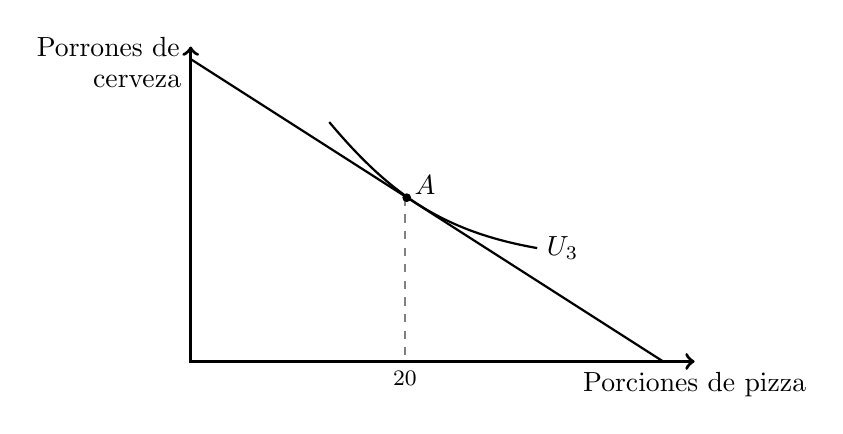
\begin{tikzpicture}[scale=0.8]
\draw[very thick,<->] (0,5) node[left]{Porrones de}--(0,0)--(8,0) node[below]{Porciones de pizza};
\node [below left] at (0,4.7) {cerveza};
\draw [thick] (2.2,3.8) to [out=310,in=170] (5.5,1.8);
\node [right] at (5.5,1.8) {$U_3$};
%\draw [thick] (0.3,4.5) to [out=290,in=165] (3.1,1.6);
%\node [right] at (3.1,1.6) {$U_2$};
\node[below] at (3.4,0) {\footnotesize 20};
%\node[below] at (0.8,0) {\footnotesize 5};
%\node[left] at (0,2.6) {\footnotesize 10};
%\node[left] at (0,3.25) {\footnotesize 15};
%\node [right] at (6,1.1) {$C$};
%\node [right] at (0.5,4.1) {$\texttt{I}$};
\draw [thick] (0,4.8) -- (7.5,0);
%\draw [thick] (0,4.8) -- (2.7,0);
%\draw[thick, dashed,gray](0.9,3.2)--(0.9,0);
\draw[thick, dashed,gray](3.4,2.6)--(3.4,0);
%\draw[thick, dashed,gray](0.9,3.25)--(0,3.25);
%\draw[thick, dashed,gray](3.43,2.6)--(0,2.6);
%\draw [thick] (0,3.3) -- (5.3,0);
%\draw[dashed](2.2,1.9)--(2.2,0);
%\node [above] at (2.4,1.9) {$C$};
%\draw[fill] (2.22,1.9) circle [radius =0.06];
%\node [above] at (3,1.7) {$\texttt{I}$};
%\node [right] at (0.8,3.5) {$B$};
%\draw[fill] (0.9,3.25) circle [radius =0.06];
\node [right] at (3.4,2.8) {$A$};
\draw[fill] (3.43,2.6) circle [radius =0.06];
\end{tikzpicture}
\end{center}
\end{figure}
\end{center}
% C8_8.png
\end{frame}

\begin{frame}
\frametitle{Cuando hay un shock en el ingreso}
\begin{itemize}
    \item Ceteris paribus: manteniendo todo lo demás constante.
    \item La restricción presupuestaria se desplaza de manera paralela hacia la derecha (con aumento de ingreso) o hacia la izquierda (con disminución de ingreso).
    \item El consumidor va a tener un conjunto factible diferente.
    \item El cambio en el ingreso no altera los precios relativos. \vspace{1mm}
    \item Habrá una nueva canasta óptima para el consumidor, que dependerá de las preferencias del individuo por los bienes en cuestión.  \vspace{1mm}
\end{itemize}
\end{frame}

%\begin{frame}{Cuando aumentan las cantidades demandadas}
% C8_4.png
%\end{frame}

%\begin{frame}{Cuando disminuyen las cantidades demandadas}
% C8_5.png
%\end{frame}

%\begin{frame}{Cuando se mantienen constantes las cantidades demandadas}
% C8_6.png
%\end{frame}

\begin{frame}
\frametitle{Cuando hay un shock en el precio de un bien}
\begin{itemize}
    \item Ceteris paribus: manteniendo todo lo demás constante.
    \item La restricción presupuestaria pivotea sobre el bien que no cambia el precio, reduciendo (aumentando) la cantidad máxima del bien afectado por el aumento (disminución) del precio.  
    \item El consumidor va a tener menos (más) canastas disponibles porque su conjunto factible se ha reducido (expandido).
    \item El cambio en el precio de un bien también altera los precios relativos. \vspace{1mm}
    \item Habrá una nueva canasta óptima para el consumidor.  \vspace{1mm}
\end{itemize}
\end{frame}

%\begin{frame}{Aumento del precio} 
% cambiar imagen a C8_7.png
%\end{frame} 

%\begin{frame}{Disminución del precio} 
% AGREGAR IMAGEN NUEVA QUE NO ESTA EN EL LIBRO
%\end{frame}

\begin{frame}
\frametitle{¿Cuál es el efecto total de un aumento en el precio de la pizza? Partimos del equilibrio A: }
\begin{center}
\begin{figure}[H]
\renewcommand{\figurename}{Figure}
\begin{center}
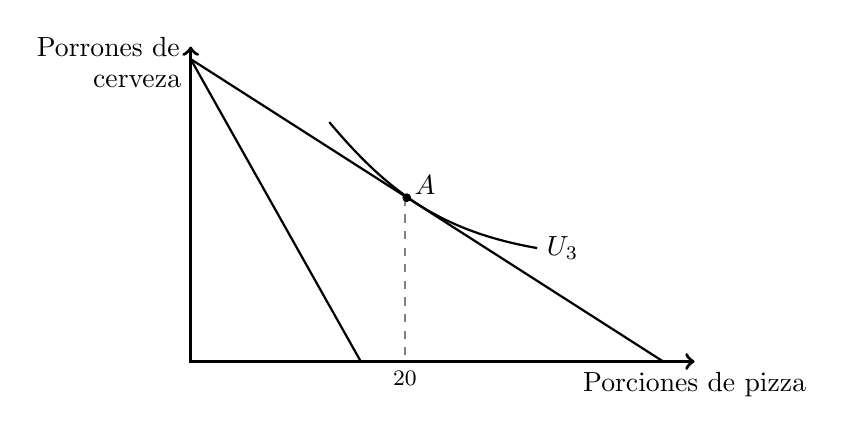
\begin{tikzpicture}[scale=0.8]
\draw[very thick,<->] (0,5) node[left]{Porrones de}--(0,0)--(8,0) node[below]{Porciones de pizza};
\node [below left] at (0,4.7) {cerveza};
\draw [thick] (2.2,3.8) to [out=310,in=170] (5.5,1.8);
\node [right] at (5.5,1.8) {$U_3$};
%\draw [thick] (0.3,4.5) to [out=290,in=165] (3.1,1.6);
%\node [right] at (3.1,1.6) {$U_2$};
\node[below] at (3.4,0) {\footnotesize 20};
%\node[below] at (0.8,0) {\footnotesize 5};
%\node[left] at (0,2.6) {\footnotesize 10};
%\node[left] at (0,3.25) {\footnotesize 15};

%\node [right] at (6,1.1) {$C$};
%\node [right] at (0.5,4.1) {$\texttt{I}$};
\draw [thick] (0,4.8) -- (7.5,0);
\draw [thick] (0,4.8) -- (2.7,0);
%\draw[thick, dashed,gray](0.9,3.2)--(0.9,0);
\draw[thick, dashed,gray](3.4,2.6)--(3.4,0);
%\draw[thick, dashed,gray](0.9,3.25)--(0,3.25);
%\draw[thick, dashed,gray](3.43,2.6)--(0,2.6);
%\draw [thick] (0,3.3) -- (5.3,0);
%\draw[dashed](2.2,1.9)--(2.2,0);
%\node [above] at (2.4,1.9) {$C$};
%\draw[fill] (2.22,1.9) circle [radius =0.06];
%\node [above] at (3,1.7) {$\texttt{I}$};
%\node [right] at (0.8,3.5) {$B$};
%\draw[fill] (0.9,3.25) circle [radius =0.06];
\node [right] at (3.4,2.8) {$A$};
\draw[fill] (3.43,2.6) circle [radius =0.06];
\end{tikzpicture}
\end{center}
\end{figure}
\end{center}
% cambiar imagen a C8_7.png
\end{frame}

\begin{frame}
\frametitle{La nueva canasta óptima es B:}
\begin{center}
\begin{figure}[H]
\renewcommand{\figurename}{Figure}
\begin{center}
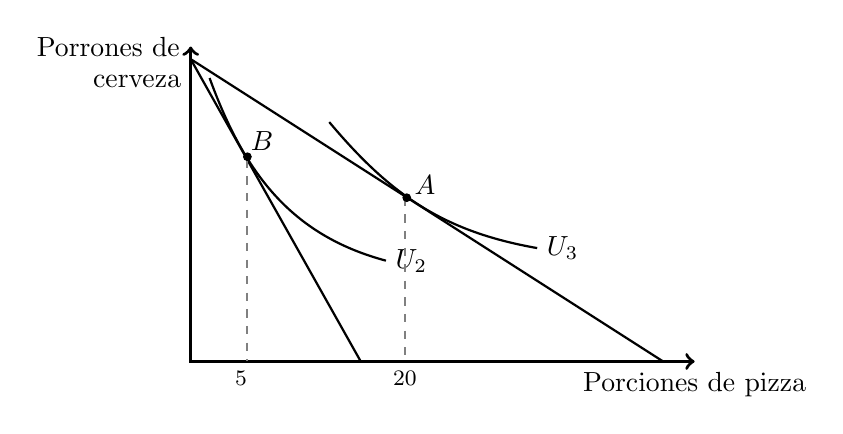
\begin{tikzpicture}[scale=0.8]
\draw[very thick,<->] (0,5) node[left]{Porrones de}--(0,0)--(8,0) node[below]{Porciones de pizza};
\node [below left] at (0,4.7) {cerveza};
\draw [thick] (2.2,3.8) to [out=310,in=170] (5.5,1.8);
\node [right] at (5.5,1.8) {$U_3$};
\draw [thick] (0.3,4.5) to [out=290,in=165] (3.1,1.6);
\node [right] at (3.1,1.6) {$U_2$};
\node[below] at (3.4,0) {\footnotesize 20};
\node[below] at (0.8,0) {\footnotesize 5};
%\node[left] at (0,2.6) {\footnotesize 10};
%\node[left] at (0,3.25) {\footnotesize 15};

%\node [right] at (6,1.1) {$C$};
%\node [right] at (0.5,4.1) {$\texttt{I}$};
\draw [thick] (0,4.8) -- (7.5,0);
\draw [thick] (0,4.8) -- (2.7,0);
\draw[thick, dashed,gray](0.9,3.2)--(0.9,0);
\draw[thick, dashed,gray](3.4,2.6)--(3.4,0);
%\draw[thick, dashed,gray](0.9,3.25)--(0,3.25);
%\draw[thick, dashed,gray](3.43,2.6)--(0,2.6);
%\draw [thick] (0,3.3) -- (5.3,0);
%\draw[dashed](2.2,1.9)--(2.2,0);
%\node [above] at (2.4,1.9) {$C$};
%\draw[fill] (2.22,1.9) circle [radius =0.06];
%\node [above] at (3,1.7) {$\texttt{I}$};
\node [right] at (0.8,3.5) {$B$};
\draw[fill] (0.9,3.25) circle [radius =0.06];
\node [right] at (3.4,2.8) {$A$};
\draw[fill] (3.43,2.6) circle [radius =0.06];
\end{tikzpicture}
\end{center}
\end{figure}
\end{center}
% cambiar imagen a C8_8.png
\end{frame}

\begin{frame}
\frametitle{El efecto total de un aumento en el precio es:} 
\begin{center}
\begin{figure}[H]
\renewcommand{\figurename}{Figure}
\begin{center}
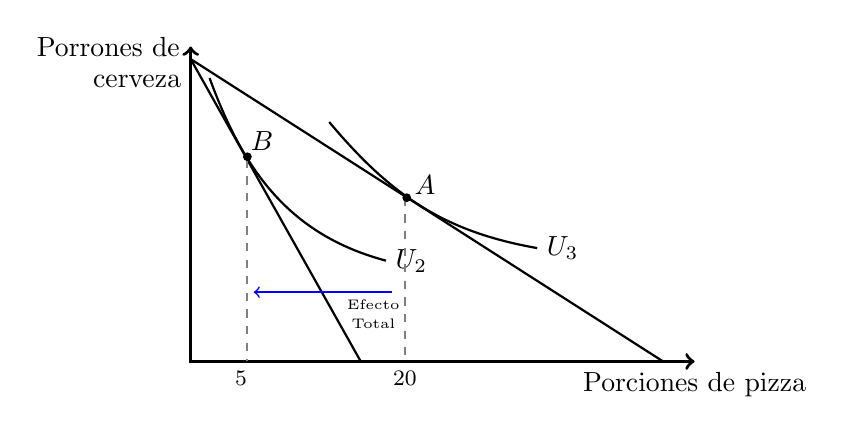
\begin{tikzpicture}[scale=0.8]
\draw[very thick,<->] (0,5) node[left]{Porrones de}--(0,0)--(8,0) node[below]{Porciones de pizza};
\node [below left] at (0,4.7) {cerveza};
\draw [thick] (2.2,3.8) to [out=310,in=170] (5.5,1.8);
\node [right] at (5.5,1.8) {$U_3$};
\draw [thick] (0.3,4.5) to [out=290,in=165] (3.1,1.6);
\node [right] at (3.1,1.6) {$U_2$};
\node[below] at (3.4,0) {\footnotesize 20};
%\node[below] at (2.22,0) {\footnotesize 10};
\node[below] at (0.8,0) {\footnotesize 5};
%\node[left] at (0,1.9) {\footnotesize 7};
%\node[left] at (0,2.6) {\footnotesize 10};
%\node[left] at (0,3.25) {\footnotesize 15};

\draw [thick] (0,4.8) -- (7.5,0);
\draw [thick] (0,4.8) -- (2.7,0);
\draw[thick, dashed,gray](0.9,3.2)--(0.9,0);
\draw[thick, dashed,gray](3.4,2.6)--(3.4,0);
%\draw[thick, dashed,gray](0.9,3.25)--(0,3.25);
%\draw[thick, dashed,gray](3.43,2.6)--(0,2.6);
%\draw[thick, dashed,gray](2.22,1.9)--(2.22,0);
%\draw[thick, dashed,gray](0,1.9)--(2.22,1.9);
%\draw [thick, gray] (0,3.3) -- (5.3,0);

\draw[semithick, blue, <-] (1,1.1)--(3.2,1.1);
\node[] at (2.9,0.9){\tiny Efecto};
\node[] at (2.9,0.6){\tiny Total};

%\draw[semithick, blue, <-] (1,1.1)--(2,1.1);
%\node[] at (1.5,0.9){\tiny Efecto};
%\node[] at (1.5,0.6){\tiny Sustitución};

%\node [above] at (2.4,1.9) {$C$};
%\draw[fill] (2.22,1.9) circle [radius =0.06];
%\node [above] at (3,1.7) {$\texttt{I}$};
\node [right] at (0.8,3.5) {$B$};
\draw[fill] (0.9,3.25) circle [radius =0.06];
\node [right] at (3.4,2.8) {$A$};
\draw[fill] (3.43,2.6) circle [radius =0.06];
\end{tikzpicture}
\end{center}
\end{figure}
\end{center}
% cambiar imagen a C8_9.png
% AGREGAR UNA FLCECHA 
%\draw[semithick, blue, <-] (1,1.1)--(3.2,1.1);
%\node[] at (2.9,0.9){\tiny Efecto};
%\node[] at (2.9,0.6){\tiny Total};
\end{frame}

\begin{frame}
\frametitle{El efecto ingreso y el efecto sustitución}
\begin{itemize}
    \item Un aumento en el precio de la pizza produce dos efectos:
    \begin{itemize}
        \item Disminuye el poder de compra, porque el consumidor tiene menor poder adquisitivo.
        \item Aumenta el costo de oportunidad de comprar cerveza.
    \end{itemize}
    \item Tenemos dos efectos
    \begin{itemize}
    \item Efecto ingreso: \\
    - La restricción presupuestaria se desplaza hacia adentro. \\
    - El efecto que el ingreso menor tendría si no hubiera cambios en el costo de oportunidad.
    \item Efecto sustitución: \\
    - La pendiente de la restricción presupuestaria (TMT) aumenta: el efecto del cambio en el costo de oportunidad, porque cambiaron los precios relativos.
    \end{itemize}
\end{itemize} 
\end{frame}

%\begin{frame}
%\frametitle{¿Cómo podemos separar estos dos efectos?} %agregar una slide de cada uno, con lo que mandamos. Agregar algunas ideas. 
%\end{frame}

\begin{frame}
\frametitle{Y si le damos menos dinero para que esté sobre $U_2$, ¿elige B?}
\begin{center}
\begin{figure}[H]
\renewcommand{\figurename}{Figure}
\begin{center}
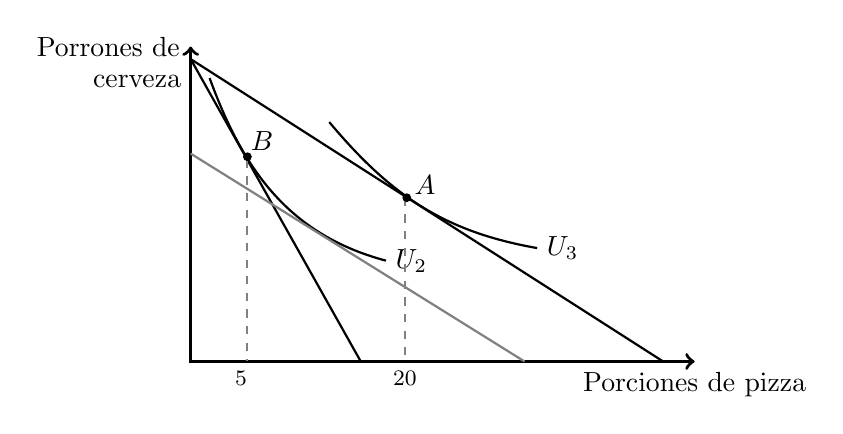
\begin{tikzpicture}[scale=0.8]
\draw[very thick,<->] (0,5) node[left]{Porrones de}--(0,0)--(8,0) node[below]{Porciones de pizza};
\node [below left] at (0,4.7) {cerveza};
\draw [thick] (2.2,3.8) to [out=310,in=170] (5.5,1.8);
\node [right] at (5.5,1.8) {$U_3$};
\draw [thick] (0.3,4.5) to [out=290,in=165] (3.1,1.6);
\node [right] at (3.1,1.6) {$U_2$};
\node[below] at (3.4,0) {\footnotesize 20};
%\node[below] at (2.22,0) {\footnotesize 10};
\node[below] at (0.8,0) {\footnotesize 5};
%\node[left] at (0,1.9) {\footnotesize 7};
%\node[left] at (0,2.6) {\footnotesize 10};
%\node[left] at (0,3.25) {\footnotesize 15};

\draw [thick] (0,4.8) -- (7.5,0);
\draw [thick] (0,4.8) -- (2.7,0);
\draw[thick, dashed,gray](0.9,3.2)--(0.9,0);
\draw[thick, dashed,gray](3.4,2.6)--(3.4,0);
%\draw[thick, dashed,gray](0.9,3.25)--(0,3.25);
%\draw[thick, dashed,gray](3.43,2.6)--(0,2.6);
%\draw[thick, dashed,gray](2.22,1.9)--(2.22,0);
%\draw[thick, dashed,gray](0,1.9)--(2.22,1.9);
\draw [thick, gray] (0,3.3) -- (5.3,0);

%\draw[semithick, blue, <-] (1,1.1)--(3.2,1.1);
%\node[] at (2.9,0.9){\tiny Efecto};
%\node[] at (2.9,0.6){\tiny Total};

%\draw[semithick, blue, <-] (1,1.1)--(2,1.1);
%\node[] at (1.5,0.9){\tiny Efecto};
%\node[] at (1.5,0.6){\tiny Sustitución};

%\node [above] at (2.4,1.9) {$C$};
%\draw[fill] (2.22,1.9) circle [radius =0.06];
%\node [above] at (3,1.7) {$\texttt{I}$};
\node [right] at (0.8,3.5) {$B$};
\draw[fill] (0.9,3.25) circle [radius =0.06];
\node [right] at (3.4,2.8) {$A$};
\draw[fill] (3.43,2.6) circle [radius =0.06];
\end{tikzpicture}
%C8_9.jpg sin el punto C marcado
\end{center}

\end{figure}
\end{center}
\end{frame}


\begin{frame}
\frametitle{No, ¡elige C!}
\begin{center}
\begin{figure}[H]
\renewcommand{\figurename}{Figure}
\begin{center}
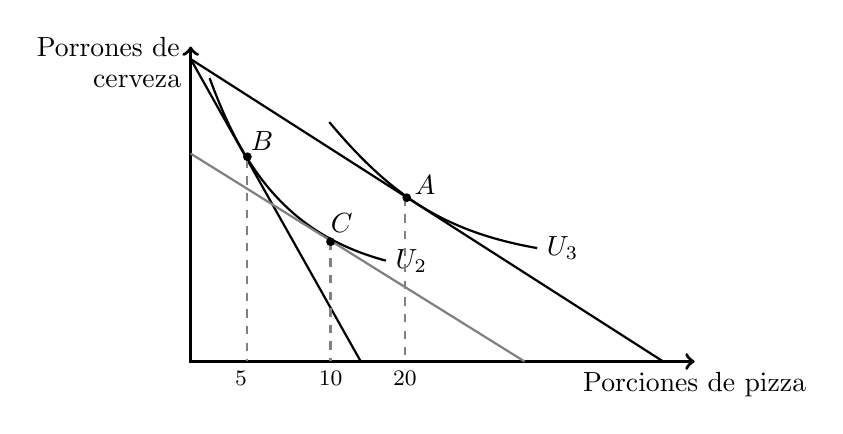
\begin{tikzpicture}[scale=0.8]
\draw[very thick,<->] (0,5) node[left]{Porrones de}--(0,0)--(8,0) node[below]{Porciones de pizza};
\node [below left] at (0,4.7) {cerveza};
\draw [thick] (2.2,3.8) to [out=310,in=170] (5.5,1.8);
\node [right] at (5.5,1.8) {$U_3$};
\draw [thick] (0.3,4.5) to [out=290,in=165] (3.1,1.6);
\node [right] at (3.1,1.6) {$U_2$};
\node[below] at (3.4,0) {\footnotesize 20};
\node[below] at (2.22,0) {\footnotesize 10};
\node[below] at (0.8,0) {\footnotesize 5};
%\node[left] at (0,1.9) {\footnotesize 7};
%\node[left] at (0,2.6) {\footnotesize 10};
%\node[left] at (0,3.25) {\footnotesize 15};

\draw [thick] (0,4.8) -- (7.5,0);
\draw [thick] (0,4.8) -- (2.7,0);
\draw[thick, dashed,gray](0.9,3.2)--(0.9,0);
\draw[thick, dashed,gray](3.4,2.6)--(3.4,0);
%\draw[thick, dashed,gray](0.9,3.25)--(0,3.25);
%\draw[thick, dashed,gray](3.43,2.6)--(0,2.6);
\draw[thick, dashed,gray](2.22,1.9)--(2.22,0);
%\draw[thick, dashed,gray](0,1.9)--(2.22,1.9);
\draw [thick, gray] (0,3.3) -- (5.3,0);

%\draw[semithick, blue, <-] (1,1.1)--(3.2,1.1);
%\node[] at (2.9,0.9){\tiny Efecto};
%\node[] at (2.9,0.6){\tiny Total};

%\draw[semithick, blue, <-] (1,1.1)--(2,1.1);
%\node[] at (1.5,0.9){\tiny Efecto};
%\node[] at (1.5,0.6){\tiny Sustitución};

\node [above] at (2.4,1.9) {$C$};
\draw[fill] (2.22,1.9) circle [radius =0.06];
%\node [above] at (3,1.7) {$\texttt{I}$};
\node [right] at (0.8,3.5) {$B$};
\draw[fill] (0.9,3.25) circle [radius =0.06];
\node [right] at (3.4,2.8) {$A$};
\draw[fill] (3.43,2.6) circle [radius =0.06];
\end{tikzpicture}
\end{center}

\end{figure}
\end{center}
\end{frame}

\begin{frame}
\frametitle{El efecto ingreso} %aclarar el gris 
\begin{center}
\begin{figure}[H]
\renewcommand{\figurename}{Figure}
\begin{center}
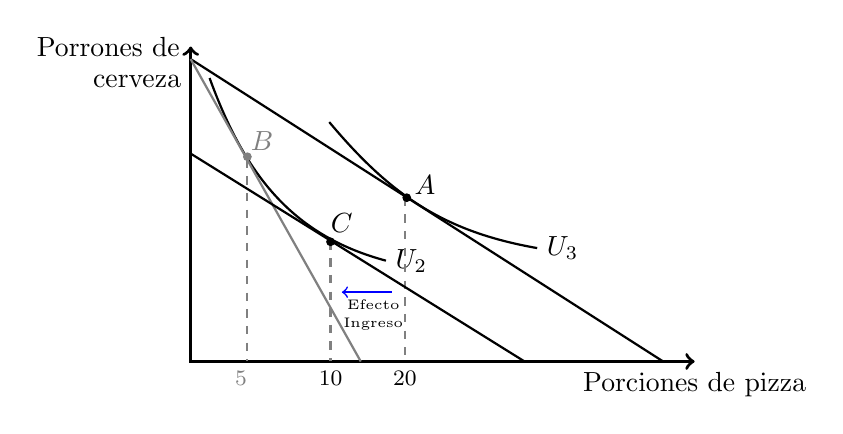
\begin{tikzpicture}[scale=0.8]
\draw[very thick,<->] (0,5) node[left]{Porrones de}--(0,0)--(8,0) node[below]{Porciones de pizza};
\node [below left] at (0,4.7) {cerveza};
\draw [thick] (2.2,3.8) to [out=310,in=170] (5.5,1.8);
\node [right] at (5.5,1.8) {$U_3$};
\draw [thick] (0.3,4.5) to [out=290,in=165] (3.1,1.6);
\node [right] at (3.1,1.6) {$U_2$};
\node[below] at (3.4,0) {\footnotesize 20};
\node[below] at (2.22,0) {\footnotesize 10};
\node[below,gray] at (0.8,0) {\footnotesize 5};
%\node[left] at (0,1.9) {\footnotesize 7};
%\node[left] at (0,2.6) {\footnotesize 10};
%\node[left] at (0,3.25) {\footnotesize 15};

\draw [thick] (0,4.8) -- (7.5,0);
\draw [thick,gray] (0,4.8) -- (2.7,0);
\draw[thick, dashed,gray](0.9,3.2)--(0.9,0);
\draw[thick, dashed,gray](3.4,2.6)--(3.4,0);
%\draw[thick, dashed,gray](0.9,3.25)--(0,3.25);
%\draw[thick, dashed,gray](3.43,2.6)--(0,2.6);
\draw[thick, dashed,gray](2.22,1.9)--(2.22,0);
%\draw[thick, dashed,gray](0,1.9)--(2.22,1.9);
\draw [thick] (0,3.3) -- (5.3,0);

%\draw[semithick, blue, <-] (1,1.1)--(3.2,1.1);
%\node[] at (2.9,0.9){\tiny Efecto};
%\node[] at (2.9,0.6){\tiny Total};

\draw[semithick, blue, <-] (2.4,1.1)--(3.2,1.1);
\node[] at (2.9,0.9){\tiny Efecto};
\node[] at (2.9,0.6){\tiny Ingreso};

%\draw[semithick, blue, <-] (1,1.1)--(2,1.1);
%\node[] at (1.5,0.9){\tiny Efecto};
%\node[] at (1.5,0.6){\tiny Sustitución};

\node [above] at (2.4,1.9) {$C$};
\draw[fill] (2.22,1.9) circle [radius =0.06];
%\node [above] at (3,1.7) {$\texttt{I}$};
\node [right,gray] at (0.8,3.5) {$B$};
\draw[fill,gray] (0.9,3.25) circle [radius =0.06];
\node [right] at (3.4,2.8) {$A$};
\draw[fill] (3.43,2.6) circle [radius =0.06];
\end{tikzpicture}
\end{center}
\end{figure}
\end{center}
\end{frame}

%\begin{frame}
%\frametitle{Pero en realidad, los precios relativos cambiaron...}
% NUEVO GRAFICO CON DOS PENDIENTES DISTINTAS Y UNA SOLA UTILIDAD
%\end{frame}

\begin{frame}
\frametitle{El efecto sustitución} %aclarar el gris
\begin{center}
\begin{figure}[H]
\renewcommand{\figurename}{Figure}
\begin{center}
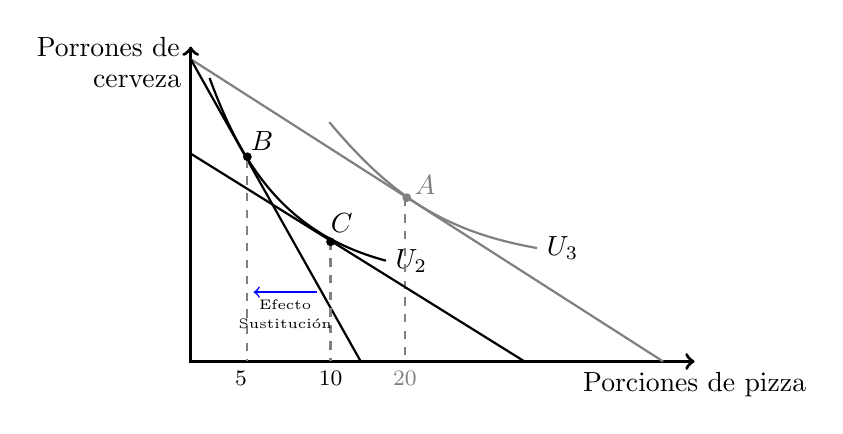
\begin{tikzpicture}[scale=0.8]
\draw[very thick,<->] (0,5) node[left]{Porrones de}--(0,0)--(8,0) node[below]{Porciones de pizza};
\node [below left] at (0,4.7) {cerveza};
\draw [thick,gray] (2.2,3.8) to [out=310,in=170] (5.5,1.8);
\node [right] at (5.5,1.8) {$U_3$};
\draw [thick] (0.3,4.5) to [out=290,in=165] (3.1,1.6);
\node [right] at (3.1,1.6) {$U_2$};
\node[below,gray] at (3.4,0) {\footnotesize 20};
\node[below] at (2.22,0) {\footnotesize 10};
\node[below] at (0.8,0) {\footnotesize 5};
%\node[left] at (0,1.9) {\footnotesize 7};
%\node[left] at (0,2.6) {\footnotesize 10};
%\node[left] at (0,3.25) {\footnotesize 15};

\draw [thick,gray] (0,4.8) -- (7.5,0);
\draw [thick] (0,4.8) -- (2.7,0);
\draw[thick, dashed,gray](0.9,3.2)--(0.9,0);
\draw[thick, dashed,gray](3.4,2.6)--(3.4,0);
%\draw[thick, dashed,gray](0.9,3.25)--(0,3.25);
%\draw[thick, dashed,gray](3.43,2.6)--(0,2.6);
\draw[thick, dashed,gray](2.22,1.9)--(2.22,0);
%\draw[thick, dashed,gray](0,1.9)--(2.22,1.9);
\draw [thick] (0,3.3) -- (5.3,0);

%\draw[semithick, blue, <-] (1,1.1)--(3.2,1.1);
%\node[] at (2.9,0.9){\tiny Efecto};
%\node[] at (2.9,0.6){\tiny Total};

%\draw[semithick, blue, <-] (2.4,1.1)--(3.2,1.1);
%\node[] at (2.9,0.9){\tiny Efecto};
%\node[] at (2.9,0.6){\tiny Ingreso};

\draw[semithick, blue, <-] (1,1.1)--(2,1.1);
\node[] at (1.5,0.9){\tiny Efecto};
\node[] at (1.5,0.6){\tiny Sustitución};

\node [above] at (2.4,1.9) {$C$};
\draw[fill] (2.22,1.9) circle [radius =0.06];
%\node [above] at (3,1.7) {$\texttt{I}$};
\node [right] at (0.8,3.5) {$B$};
\draw[fill] (0.9,3.25) circle [radius =0.06];
\node [right,gray] at (3.4,2.8) {$A$};
\draw[fill,gray] (3.43,2.6) circle [radius =0.06];
\end{tikzpicture}
\end{center}
\end{figure}
\end{center}
\end{frame}


\begin{frame}
\frametitle{La suma del efecto sustitución y el efecto ingreso nos da el efecto total} %aclarar el gris
\begin{center}
\begin{figure}[H]
\renewcommand{\figurename}{Figure}
\begin{center}
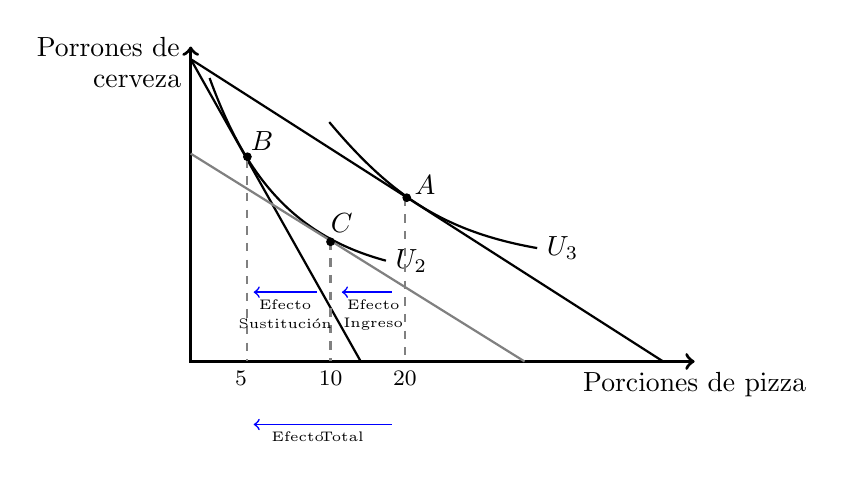
\begin{tikzpicture}[scale=0.8]
\draw[very thick,<->] (0,5) node[left]{Porrones de}--(0,0)--(8,0) node[below]{Porciones de pizza};
\node [below left] at (0,4.7) {cerveza};
\draw [thick] (2.2,3.8) to [out=310,in=170] (5.5,1.8);
\node [right] at (5.5,1.8) {$U_3$};
\draw [thick] (0.3,4.5) to [out=290,in=165] (3.1,1.6);
\node [right] at (3.1,1.6) {$U_2$};
\node[below] at (3.4,0) {\footnotesize 20};
\node[below] at (2.22,0) {\footnotesize 10};
\node[below] at (0.8,0) {\footnotesize 5};
%\node[left] at (0,1.9) {\footnotesize 7};
%\node[left] at (0,2.6) {\footnotesize 10};
%\node[left] at (0,3.25) {\footnotesize 15};

\draw [thick] (0,4.8) -- (7.5,0);
\draw [thick] (0,4.8) -- (2.7,0);
\draw[thick, dashed,gray](0.9,3.2)--(0.9,0);
\draw[thick, dashed,gray](3.4,2.6)--(3.4,0);
%\draw[thick, dashed,gray](0.9,3.25)--(0,3.25);
%\draw[thick, dashed,gray](3.43,2.6)--(0,2.6);
\draw[thick, dashed,gray](2.22,1.9)--(2.22,0);
%\draw[thick, dashed,gray](0,1.9)--(2.22,1.9);
\draw [thick, gray] (0,3.3) -- (5.3,0);

\draw[semithick, blue, <-] (1,-1)--(3.2,-1);
\node[] at (1.7,-1.2){\tiny Efecto};
\node[] at (2.4,-1.2){\tiny Total};

\draw[semithick, blue, <-] (2.4,1.1)--(3.2,1.1);
\node[] at (2.9,0.9){\tiny Efecto};
\node[] at (2.9,0.6){\tiny Ingreso};

\draw[semithick, blue, <-] (1,1.1)--(2,1.1);
\node[] at (1.5,0.9){\tiny Efecto};
\node[] at (1.5,0.6){\tiny Sustitución};

\node [above] at (2.4,1.9) {$C$};
\draw[fill] (2.22,1.9) circle [radius =0.06];
%\node [above] at (3,1.7) {$\texttt{I}$};
\node [right] at (0.8,3.5) {$B$};
\draw[fill] (0.9,3.25) circle [radius =0.06];
\node [right] at (3.4,2.8) {$A$};
\draw[fill] (3.43,2.6) circle [radius =0.06];
\end{tikzpicture}
\end{center}
\end{figure}
\end{center}
\end{frame}

\end{document}

